
Masinnägemine on tehisintellekti valdkond, mis tegeleb digitaliseeritud visuaalsest materjalist (fotod, videod) inimesele arusaadava ning vajaliku informatsiooni eraldamisega ning seejärel otsuste tegemisega saadud info põhjal, kasutades arvuteid. Kui tehisintellekt annab arvutitele võime mõelda, siis masinnägemine annab neile võimekuse näha, vaadelda ja mõista ümbritsevat keskkonda.

Masinnägemine toimib sarnaselt inimese nägemisele, kuid inimestel on selles astmes eluaegne edumaa, nad õpivad objekte eristama juba sünnist saati. Inimene on võimeline elu jooksul eristama mitmeid objekte, nende kaugust, nende statsionaarsust või dünaamilisust ning tuvastama vigu piltidel või objektidel.

Masinnägemise puhul ``treenitakse'' arvuteid, et viia läbi sarnaseid operatsioone, kuid seda palju lühema ajaga, kasutades kaameraid, massiivseid andmehulki ning algoritme inimsilma võrkkesta, optiliste närvide ja aju nägemise interpreteerimise asemel. Antud süsteemil on ka eelisi inimnägemise ees, milleks on spetsialiseerumine. Kui õpetame süsteemile selgeks, milline näeb välja laev ja poi, siis valminud tuvastusmudel on võimeline analüüsima mitmeid sadu objekte ja olukordi sekundis ning vastavalt ka reageerima palju suurema täpsuse-, kindluse- ja kiirusega kui inimene, kes tegeleks sama operatsiooniga.

Masinnägemine on kasutusel mitmetes valdkondades: energiahaldus (tarbimisprognoosid), tootmine (toodete defektide kontroll) ja autotööstus (autonoomsed sõidukid ja juhiabisüsteemid) ning nõudlus masinnägemise spetsialistidele on kasvuteel {[}14{]}.

\section{Masinnägemise tööpõhimõte}\label{masinnuxe4gemise-tuxf6uxf6puxf5himuxf5te}

Masinnägemise mudeli treenimiseks ning loomiseks on vaja massiivset andmehulka, mida analüüsitakse mitmeid tuhandeid kordi seni, kuni mudel leiab andmetest seaduspärasusi, mustreid ning objektide puhul iseloomulikke kujundeid, mis lõpuks võimaldavad iseseisvalt uutelt, seni nägemata piltidelt otsitavat objekti tuvastada.

Antud toimingu läbiviimiseks kasutatakse masinõpet, mille üheks osaks on tehisnärvivõrgud ning selle alamosadest täpsemalt süvaõpet ja konvolutsioonilisi närvivõrke.

Masinõppe puhul kasutatakse algoritmilisi mudeleid, mis võimaldavad arvutil aru saada visuaalsete andmete sisust. Piisava hulga andmete edastamisel mudelile suudab arvuti endale andmete põhjal selgeks teha, millega on pildil tegemist ning mis on piltide erinevused. Algoritmid võimaldavad masinal iseseisvalt õppida, mis on oluliselt efektiivsem kui see, et inimene eelprogrammerib arvuti pilte tuvastama.

Konvolutsiooniline tehisnärvivõrk aitab masinnägemise mudelil pildist aru saada, vaadates sisendit mitmete väiksemate, sildistatud aladena. Sildistatud aladel tehakse konvolutsioonilisi operatsioone, mille alusel närvivõrk teeb ennustusi selle kohta, mida ta näeb. Närvivõrk kordab neid operatsioone ning kontrollib ennustuste täpsust iteratiivselt seni, kuni saadud tulemid on vajaliku täpsusega ning tõesed. Pärast taolise operatsiooni edukat kulgemist on mudel võimeline nägema ja tuvastama pilte inimesele arusaadavas formaadis {[}14{]}.

\section{Konvolutsiooniline närvivõrk}\label{konvolutsiooniline-nuxe4rvivuxf5rk}

Konvolutsioonilise närvivõrgu (\emph{Convolutional Neural Network, ConvNet, CNN}) puhul on tegemist süvaõppealgoritmiga, mis suudab sisendiks antud pildilt leida sellele iseloomulikud omadused ning neid üksteisest eristada. Võrreldes teiste pildituvastusalgoritmidega, on CNNi jaoks vajalik pildi eeltöötluse maht oluliselt väiksem. Samuti on CNN võimeline iseseisvalt piisava hulga treenimisega piltide omaduste eristamiseks filtreid looma (piltide eripärasid selgeks õppima), erinevalt käsitsi häälestatavatest algoritmidest, mis seda nii täpselt teha ei võimalda. {[}15{]}

Antud närvivõrku eristavad teistest võrkudest kihid, mis on antud võrgu alustaladeks:

\begin{itemize}
\item
  Konvolutsiooniline kiht (\emph{Convolutional layer})
\item
  Skaleerimise/ahendamise kiht (\emph{Pooling layer})
\item
  Täielikult ühendatud kiht (\emph{Fully Connected layer})
\end{itemize}

Konvolutsiooniline kiht on CNNi esimene kiht, täielikult ühendatud kiht on viimane, skaleerimine ning täiendavad kihid asetsevad nende vahel. Iga järgneva kihiga suureneb närvivõrgu kompleksus ning täieneb ka süsteemi arusaam sisendiks antud pildist. Ülemised kihid mõistavad lihtsamaid omadusi nagu näiteks värvid ja servad. Sügavamates kihtides tekib süsteemil generaliseeritum arusaam pildil olevatest elementidest või kujutistest ning saadud info põhjal, eeldusel, et seda on piisavalt, teeb süsteem otsuse, millega on fotol tegemist.

\textbf{Konvolutsiooniline} kiht (\emph{convolutional layer}) on CNNi olulisim osa närvivõrgus, milles toimub kõige suurem hulk arvutusi. Antud kiht vajab sisendinfot, filtrit ja tunnusjoonte kaarti (\emph{feature map}). Eeldame et sisendina on tegemist värvilise pildiga, mis on kolme dimensioonilise maatriksi kujul (roheline, punane, sinine -- kolm kanalit, kõrgus, laius, sügavus -- kolm dimensiooni). Sellega on sisendandmed määratud. Samuti on meil tarvis ka tunnusjoonte tuvastusfunktsiooni ehk kernelit ehk \textbf{filtrit}, mis liigub astmeliselt üle andmete ning kontrollib kas teatud omadus eksisteerib pildil ning sooritab ka sellekohased arvutused. Eelnevalt kirjeldatud operatsioon on konvolutsioon.

\textbf{Filtri} puhul on tegemist kahedimensioonilise, konstantsete kaaludega täidetud maatriksiga, mis esindab pildi osa. Filtreid on erinevates suurustes, kuid traditsiooniliselt on nad kolm korda kolm maatriksina. Pildi osale rakendatakse filter, mille tulemuseks on pildi ala maatriksi ning filtri maatriksi skalaarkorrutis, mis antakse edasi väljundmaatriksi. Seejärel nihkub filtri maatriks ette määratud pikslite arvu võrra edasi, kuni terve pildiga on antud operatsioon tehtud ning mille tulemusena on saadud konvolutsiooniliste tunnuste kaart (vt Joonis 2.2.1).

\begin{figure}
\centering
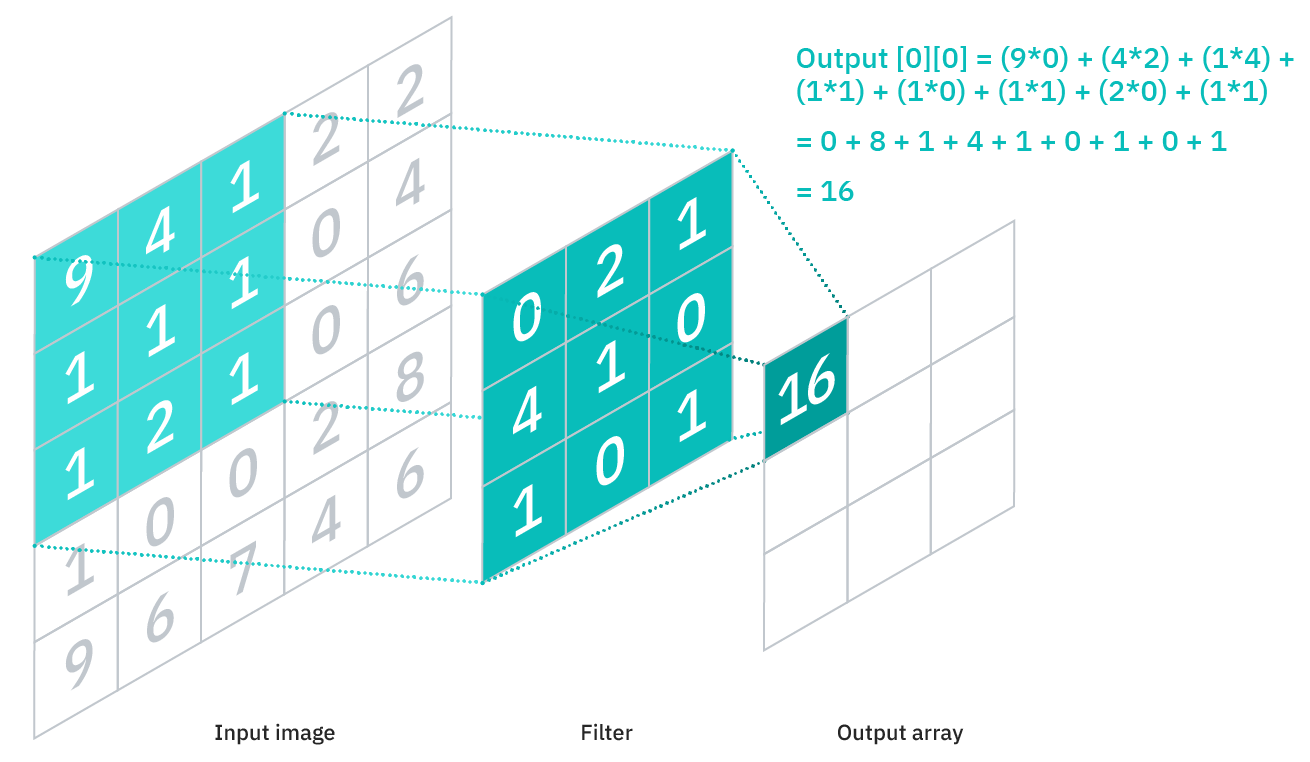
\includegraphics[width=6.10174in,height=3.55556in,alt={matrix multiplication in convolutional neural networks}]{media/image5.png}
\caption{matrix multiplication in convolutional neural networks}
\end{figure}

Joonis 2.2.1. Maatrikskujul pildil (vasakul) tehakse operatsioon filtriga (keskel), mis annab tulemuseks skalaarkorrutise tunnuste kaardina (paremal)

Joonist vaadeldes näeme, et väljundmaatriksis vastab üks argument mitmele sisendpikslile ehk antud operatsiooni puhul konvolutsiooniline kiht ja ka järgnevalt arutatav skaleerimise kiht kuuluvad osaliselt ühendatud närvivõrgu kihtide hulka. Pärast iga konvolutsioonilist operatsiooni toimub tunnuste kaardi protsesseerimine ReLU {[}16{]} aktiveerimise funktsiooni kihis ning seejärel saadetakse saadud väljundid \textbf{skaleerimise} kihti.

\textbf{Skaleerimise} kiht (\emph{pooling layer}) tegeleb sisendi alla skaleerimisega vähendades seetõttu ka sisendparameetrite arvu, suurendades närvivõrgu efektiivsust ning vähendades võrgu ületreenimise riski. Sarnaselt konvolutsioonilise kihi operatsioonidele, toimub ka siin töötlus kogu pildi peal, ainukese erinevusena konvolutsioonist, puuduvad selle kihi filtril kaalud. Antud kihis on võimalik teha maksimaalset skaleerimist (\emph{max pooling}) ja keskmistatud skaleerimist (\emph{average pooling}). Esimesel puhul toimub filtri liikumisel üle pildi maksimaalse väärtusega piksli valik, mis saadetakse väljundmaatriksisse, teisel puhul arvutatakse filtri liikumisel üle pildi pikslite keskmine väärtus, mis väljundmaatriksisse edastatakse. Maksimaalset skaleerimist kasutatakse rohkem kui keskmistatud skaleerimist.

\textbf{Täielikult ühendatud} kiht (\emph{fully connected layer}) tegeleb eelmistest kihtidest kogutud ja filtreeritud info klassifitseerimisega. Antud kiht kasutab softmax {[}17{]} aktiveerimisfunktsiooni sisendite korrektseks klassifitseerimiseks, väljastades igale klassile tõenäosuse hinnangu, kus kõikide klasside hinnangute summa on üks (vt Joonis 2.2.2). {[}18{]}

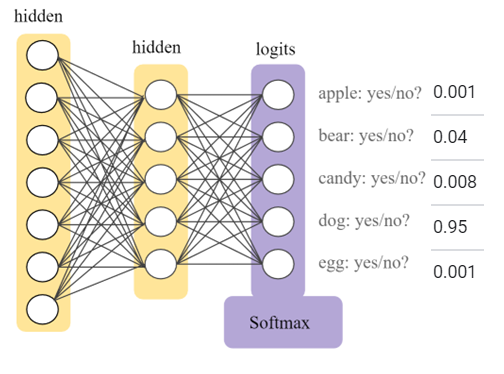
\includegraphics[width=5.25073in,height=3.89638in]{media/image6.png}

Joonis 2.2.2. SoftMaxi funktsiooniga rakendatud väljundite kiht närvivõrgus (lilla) ja tõenäosused iga klassi kohta (paremal) {[}17{]}
